\scanpage{71}
% archive sheet number: 70

of \inserted{(iso)}\handwritten{
\begin{tikzpicture}[x=1cm,y=1cm,baseline=-.1cm]\draw[thin] (0,-.25).. controls (-.15,0) and (0,.18)..(.38,.15).. controls (.9,.1) and (1.05,.4)..(1.05,.65);\draw[gray,thin] (.02,-.26).. controls (-.07,0) and (.05,.12)..(.35,.12);\end{tikzpicture}}motives \inserted{(semisimple)}\handwritten{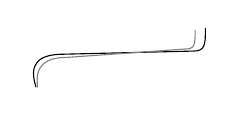
\begin{tikzpicture}[x=1cm,y=1cm,baseline=-.1cm]\draw[thin] (0,-.3).. controls (-.1,0) and (.03,.12)..(.35,.12)--(2,.16).. controls (2.15,.16) and (2.15,.25)..(2.15,.45);\draw[gray,thin] (.02,-.3).. controls (-.02,-.02) and (.12,.08)..(.4,.08)--(1.95,.19).. controls (2.02,.2) and (2.02,.3)..(2.02,.43);\end{tikzpicture}} over $k$, and the subscript $\underline{Q}_p$ denotes th\unsure{\deleted{'}e|'e} \deleted{effect of the} base change by $\underline{Q}\handwritten{\longrightarrow}\underline{Q}_p$ . This homomorphism is compatible with the ``Tate'' augmentation and with the effectivity structures. Modulo some work to be done by Berthelo\handwritten{t}, for $k=\handwritten{\mathbb{F}}_q$ a finite field with $q$ elements, knowledge of the image \deleted{of $X$ \unsure{q|i}\unsure{n}} $H^*(X)$ in $\mathrm{Fcriso}(k)$ makes it possible to calculate \unsure{\deleted{its}the|\deleted{the}its} function $\handwritten{\zeta_X}$ of $X$, by the formula which one guesses and which I am preparing to describe. (Besides, modulo the Weil conjectures, knowledge of the function $\handwritten{\zeta_X}$ makes it possible, thanks to this formula, to reconstruct $H^{\handwritten{*}}_{\mathrm{cris}}(X)$ up to isomorphism in $\mathrm{Fcriso}(k)$, at least virtually (i.e. the image of each $H^i_{\mathrm{cris}}(X)$ in the ring $K(\mathrm{Fcriso}(k)))$ if one does not wish to admit that \deleted{\unsure{l|t}\unsure{t|i|o}\unsure{o|u}\unsure{b|u|s}} the $H^i$ are necessarily semisimple elements of $\mathrm{Fcriso}(k)$....)

\handwritten{5.} F-\uline{crystals of \deleted{level} slope zero}. We shall define further on the \uline{slope} of a ``homogeneous'' F-crystal. Here, we are going to \unsure{\deleted{o}i|\deleted{i}o}ntroduce directly the F-crystals of slope zero. For this, for every constructible $p$-adic sheaf \inserted{$V$}\handwritten{\begin{tikzpicture}[x=1cm,y=1cm,baseline=0cm]\draw[thin] (0,-.25).. controls (-.1,-.05) and (.3,.3)..(.4,.7);\end{tikzpicture}} on $k$\handwritten{(}thus corresponding to a continuous \deleted{repr\unsure{e|e}sentatio}n\inserted{action} of $\handwritten{\pi}=\operatorname{Gal}(\handwritten{\bar{k}}/k)$ on a finitely generated module over $\underline{Z}_p$) one associates to it in an obvious \deleted{\unsure{d|q}}\handwritten{w}ay an F-crystal $M$, sometimes denoted (by abuse of notation)
\[
M=\unsure{\mathbb{V}|\mathbb{M}|\mathbb{F}}\otimes_{\underline{Z}_p}W\ ,
\]
(even if there is no chosen $W$, in the case $k$ imperfect \handwritten{!} ), \unsure{\deleted{o}O|\deleted{O}o|6}ne will have :

\margin{\handwritten{\figure{
\begin{tikzpicture}\draw (0,0) -- (0.02,0.7) -- (0,1.6);\end{tikzpicture}}}}
\uline{Proposition}\handwritten{5\unsure{,|.}1.} The functor $\mathbb{M}\handwritten{\mathrel{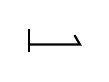
\begin{tikzpicture}[x=1cm,y=1cm,baseline=-.04cm]\draw[thick] (0,-.1)--(0,.2);\draw[thick] (0,0)--(.65,0)--(.58,.12);\end{tikzpicture}}}V\otimes_{\underline{Z}_p}W$ is an equivalence from the category of constructible $p$-adic sheaves\handwritten{\begin{tikzpicture}[x=1cm,y=1cm,baseline=0cm]\draw[thin] (0,-.3).. controls (.13,-.2) and (.14,.1)..(.26,.55);\end{tikzpicture}}on $k$ to the full subcategory of the category of F-crystals \unsure{\deleted{d}o|\deleted{s}d}\unsure{\deleted{a}ve|\deleted{u}a|\deleted{e}ve|\deleted{u}e}r $k$, consisting of the F-crystals $M$ such that $F_M : M^{\handwritten{\unsure{\deleted{\sigma}\sigma|\sigma}}}\handwritten{\longrightarrow}M$ is an \uline{isomorphism} .

\uline{Corollary}\handwritten{5.\unsure{2|1}.} The preceding functor induces a fully faithful functor (compatible with the $\otimes$-structures)\inserted{\handwritten{$i$}}\handwritten{\begin{tikzpicture}[x=1cm,y=1cm,baseline=0cm]\draw[thin] (0,-.3).. controls (-.1,-.02) and (.2,.25)..(.5,.33).. controls (.7,.35) and (.85,.38)..(.95,.5);\end{tikzpicture}} from the category of

\mspage{70}
